% ===================================================================
% Preprint Title: A 3D Mathematical Model of a Dynamically Coupled Field...
% Author: Toshiya Konno
% Version: 3.0 (Date: 2025-07-14)
% This is the final, peer-reviewed quality source code for publication.
% All critical and important revisions are incorporated.
% ===================================================================

\documentclass[a4paper,11pt,ja=standard]{bxjsarticle}

% ---------- Packages ----------
\usepackage{fontspec}
\usepackage{amsmath,amssymb,amsfonts}
\usepackage{graphicx}
\usepackage{geometry}
\usepackage{hyperref}
\usepackage{authblk}
\usepackage{placeins}
\usepackage{caption}
% ---------- PDF Metadata ----------
\hypersetup{
  pdftitle={A 3D Mathematical Model of a Dynamically Coupled Field Inspired by Operator Algebras (Version 3.0)},
  pdfauthor={Toshiya Konno},
  pdfsubject={We demonstrate that the stable coupled motion in our model exhibits remarkable robustness against strong dissipation, undergoing a sharp, first-order-like phase transition at a critical damping threshold. This finding significantly strengthens the hypothesis that our model captures an essential feature of robust information transfer in complex, noisy environments.},
  pdfkeywords={Coupled Gross–Pitaevskii Equations; Quantum-Classical Hybrid System; Tensegrity; Soliton Dynamics; Topological Robustness; Dissipation; Phase Transition},
  pdfcreator={XeLaTeX (TeX Live)},
  pdflang={en}
}

% ---------- Fonts (for local compilation) ----------
% Note: These fonts may not be available on platforms like arXiv.
% For submission, compiling to a final PDF locally is recommended.
\setmainfont{TeX Gyre Termes}
\setjamainfont{IPAexMincho}
\setsansfont{IPAexGothic}

% ---------- Layout ----------
\geometry{left=25mm,right=25mm,top=25mm,bottom=25mm}

% ---------- Title, Author, Date ----------
\title{作用素環論に着想を得た動的結合場の3次元数式モデル\\
\large A 3D Mathematical Model of a Dynamically Coupled Field Inspired by Operator Algebras: Theoretical Foundation and Numerical Verification of Stable Coupled Motion}
\author[1]{今野聖也\,Toshiya Konno}
\affil[1]{Independent Researcher\\\href{mailto:ktlifeisonlyreallyoverafter60@gmail.com}{ktlifeisonlyreallyoverafter60@gmail.com}}
\date{2025年7月14日(Version 3.0)}

\begin{document}
\maketitle

\noindent\textbf{Keywords:}\ Coupled Gross–Pitaevskii Equations; Quantum-Classical Hybrid System; Tensegrity; Soliton Dynamics; Topological Robustness; Operator Algebras

% ---------- Abstract (Japanese) ----------
\begin{abstract}
\noindent 本稿では、量子場と古典的構造体の動的相互作用を記述する、新たな3次元数式モデルを提案する。本モデルは、作用素環論の思想に基づき、量子場と古典場がヘルマン–ファインマン力と自己復元力を介して結合する自己無撞着な系として構築される。我々は数値シミュレーションを通じて、情報キャリアである量子ソリトンが古典構造体と一体となって安定的に移動する「安定結合移動」という現象を観察・解析した。さらに本稿では、この現象の物理的妥当性を深く検証するため、系に散逸(抵抗)を導入する。その結果、この安定状態が強い散逸に対しても極めて頑健であること、そしてある臨界値で一次相転移的な崩壊を示すという、新たな核心的性質を明らかにした。この頑健な結合状態は、細胞内のような複雑な環境におけるロスレスな情報伝達機構を理解する上で、新たな理論的枠組みを提供する可能性がある。
\end{abstract}

% ---------- Abstract (English) ----------
\vspace{1em}
\noindent\textbf{Abstract}
\par\noindent
\small
We propose a three-dimensional mathematical model that dynamically couples a quantum field and a single-degree-of-freedom classical barrier, inspired by operator-algebraic ideas. The quantum part is governed by a non-linear Gross–Pitaevskii equation, whereas the barrier follows Newtonian dynamics with a Hellmann–Feynman feedback force and a tensegrity-like restoring force. Through numerical simulations, we observed and analyzed a \emph{stable coupled motion}, where a self-trapped quantum soliton travels together with the barrier. Furthermore, to investigate its physical relevance, we introduce dissipation into the system. We demonstrate that this state exhibits remarkable robustness against strong dissipation and reveal a key new feature: a sharp, first-order-like phase transition at a critical damping threshold. This robust coupled state may provide a new theoretical framework for understanding loss-less information transport in complex environments such as intracellular processes.
\vspace{2em}

\FloatBarrier
% ===============================================================
\section{導入 (Introduction)}
% ---------------------------------------------------------------
生命の基本単位である細胞は、その内部において、熱揺らぎや粘性による散逸が支配的な環境下にありながら、驚くほど効率的で、かつ正確な情報伝達を行っている。この一見矛盾した現象を説明するため、我々は細胞骨格が持つ「テンセグリティ構造」の安定性と、量子現象に見られる「トポロジカルな保護」の頑健性に着目した。本研究の目的は、これらの概念を統一的に記述する新たな物理モデルを構築し、量子的な情報キャリアが古典的な構造体と結合することで、情報をロスなく安定的に輸送するメカニズムが存在しうることを、理論とシミュレーションの両面から検証することである。

以前の研究(Version 2.5)では、我々は散逸のない理想的な系において、この「安定結合移動」の存在を初めて報告した。しかし、細胞内のような現実の生物物理学的環境は、水の粘性などによる散逸が不可避的に存在する。したがって、本モデルの物理的妥当性を真に評価するためには、この安定状態が散逸に対してどの程度の頑健性を持つかを検証することが不可欠である。そこで本稿では、モデルに粘性抵抗項を導入し、散逸環境下における系のダイナミクスを詳細に解析する。
\FloatBarrier
% ===============================================================
\section{モデル本体 (The Model)}
% ---------------------------------------------------------------
\subsection{基本方程式系}
本モデルは、量子場 $\psi(\mathbf{r},t)$(GP波動関数)と、1自由度の古典場 $u(t)$(障壁の中心位置 $z_b(t)$)の動的な相互作用を記述する。古典場には、環境との相互作用をモデル化するための散逸項が含まれており、系全体は以下の連成方程式系によって定義される。
\begin{align}
 i\hbar\frac{\partial\psi(\mathbf r,t)}{\partial t}&=H[u(t)]\psi(\mathbf r,t), \label{eq:schrodinger} \\
  M\frac{d^{2}u(t)}{dt^{2}}&=F_{\text{feedback}}[\psi,u]+F_{\text{restoring}}[u] - \gamma \frac{du(t)}{dt}. \label{eq:newton_diss}
\end{align}

\subsection{ハミルトニアンと力の具体的定義}
\paragraph{全ハミルトニアン}
\[
H=-\frac{\hbar^{2}}{2m}\nabla^{2}+V_{\text{trap}}(\mathbf r)+V_{\text{barrier}}(\mathbf r,u(t))+g|\psi|^{2}.
\]
\paragraph{外部ポテンシャル}
\[
V_{\text{ext}}(\mathbf r,u)=V_{\text{trap}}(\mathbf r)+V_{\text{barrier}}(\mathbf r,u),\quad\mathbf r=(x,y,z).
\]
\begin{itemize}
\item 横方向閉じ込め:
      \[
         V_{\text{trap}}(\mathbf r)=
         \tfrac{1}{2} m\omega_{\perp}^{2}\bigl(x^{2}+y^{2}\bigr).
      \]
\item 動的障壁:
      \[
         V_{\text{barrier}}(\mathbf r,u(t))
           = A \exp\!\left[
               -\frac{\bigl(z-z_b(t)\bigr)^{2}}{2\sigma^{2}}
             \right].
      \]
\end{itemize}
\noindent
(シミュレーションでは、無次元化された振幅 $A=0.1$, 幅 $\sigma=4.0$ を使用)

\paragraph{フィードバック力(Hellmann–Feynman力)}
\[
F_{\text{feedback}}=-\!\int\psi^{*}(\mathbf r,t)\,
      \frac{\partial V_{\text{barrier}}}{\partial z_b}\,
      \psi(\mathbf r,t)\,d^{3}\mathbf r.
\]

\paragraph{自己復元力(テンセグリティ構造の表現)}
\[
 F_{\text{restoring}}=-k_{\text{mech}}\bigl(z_b(t)-z_{b,0}\bigr),\qquad
 k_{\text{mech}}>0.
\]

\paragraph{非線形相互作用}
本モデルでは、ソリトンの自己束縛を可能にするため、引力相互作用 $g<0$ を仮定する。(シミュレーションでは無次元化された有効相互作用強度 $g = -15.0$ を使用)。3次元空間における引力相互作用系の崩壊は、強い横方向閉じ込めポテンシャル $V_{\text{trap}}$ によって系が実効的に準1次元化されるため、本研究で扱った粒子数の範囲では抑制される。

\subsection{モデルが記述する核心的物理現象}
本モデルは、一連の数値シミュレーションを通じて「安定結合移動 (Stable Coupled Motion)」という核心的現象をサポートすることを、観察・解析した。この現象は、量子場ソリトンがその局在した形状を維持したまま、古典場(障壁)と一体となって安定的に移動する状態である。
\begin{itemize}
    \item \textbf{存在条件:}
    本研究で用いたパラメータ群(Table \ref{tab:params}参照)において、この安定結合移動は、無次元化された初期運動量 $k_{z,\text{kick}}$ が臨界領域 $0.1 < k_{z,\text{kick}} \leq 0.15$ にある場合に観測された。(ここで、$k_{z,\text{kick}}$ は初期運動量を $\hbar$ で割った波数 $\Delta p_z/\hbar$ に相当する)

    \item \textbf{ロバスト性 (Robustness):}
    この現象は、上記パラメータ領域内において、系に加えられる外部からのランダムノイズに対しても安定性を維持する、極めて頑健なものである。これは、情報が散逸・破壊されることなく、保護されながら伝達される「ロスレス情報伝達」のメカニズムを示唆する。
\end{itemize}

\noindent
なお、本研究で観測されたソリトンと障壁の軌跡は、激しい内部振動を伴うため、単純な線形相関分析では、その強い結合性を見出すことはできない。この系のダイナミクスを完全に理解するには、その非線形な特性を考慮した、より高度な時系列解析が必要である。本稿では、まず、この現象の存在を報告することに主眼を置く。

\begin{table}[h!]
\centering
\caption{Key symbols and simulation parameters.}
\label{tab:params}
\begin{tabular}{l l c}
\hline\hline
Symbol & Meaning & Value (dimensionless) \\ \hline
$\psi$ & Quantum field wave function & – \\
$u$ ($z_b$) & Classical field displacement & – \\
$A$ & Barrier potential amplitude & 0.1 \\
$\sigma$ & Barrier potential width & 4.0 \\
$g$ & Nonlinear interaction strength & -15.0 \\
$k_{\text{mech}}$ & Restoring force spring constant & 10.0 \\
$M$ & Effective mass of the classical field & 50.0 (Standard) \\
$k_{z,\text{kick}}$ & Initial momentum (wavenumber) & 0.15 (Standard) \\
$\gamma$ & Damping coefficient & 0.0 -- 2.0 (swept) \\ \hline\hline
\end{tabular}
\end{table}

\FloatBarrier
\section{補遺 (Supplementary Information) - モデルの妥当性と限界}

\subsection{無次元化と物理スケール}
本研究のシミュレーションは、現象の普遍性を探るため無次元化単位系で行われた。
\begin{quote}
\textbf{Example Mapping: スケール変換例} \\
無次元化 $\tilde t = t/t_0, \tilde{\mathbf{r}} = \mathbf{r}/\ell_0$ において、典型的なBEC実験のパラメータ(Na-23原子、$\ell_0 = 1\,\mu\text{m}$, $t_0 = 1\,\text{ms}$)を仮定した場合、シミュレーション時間 $t=40.0$ は実時間で 40 ms に相当する。
\end{quote}

\subsection{数値計算手法と誤差評価}
時間発展には標準的なSplit-step Fourier法を用い、計算空間には全方向に周期境界条件を課した。(計算格子サイズ: $N_x=N_y=64, N_z=256$)。理想的な散逸なし系におけるエネルギー保存則の検証(Figure \ref{fig:conservation})では、時間ステップ $\Delta t = 5\times10^{-6}$ を用いた。一方、本稿の主要なテーマである散逸系のダイナミクス解析(Figure \ref{fig:dissipation})では、現象の安定性を確認するため、時間ステップ $\Delta t = 0.0005$ で計算を実行した。

\begin{figure}[h!]
  \centering
  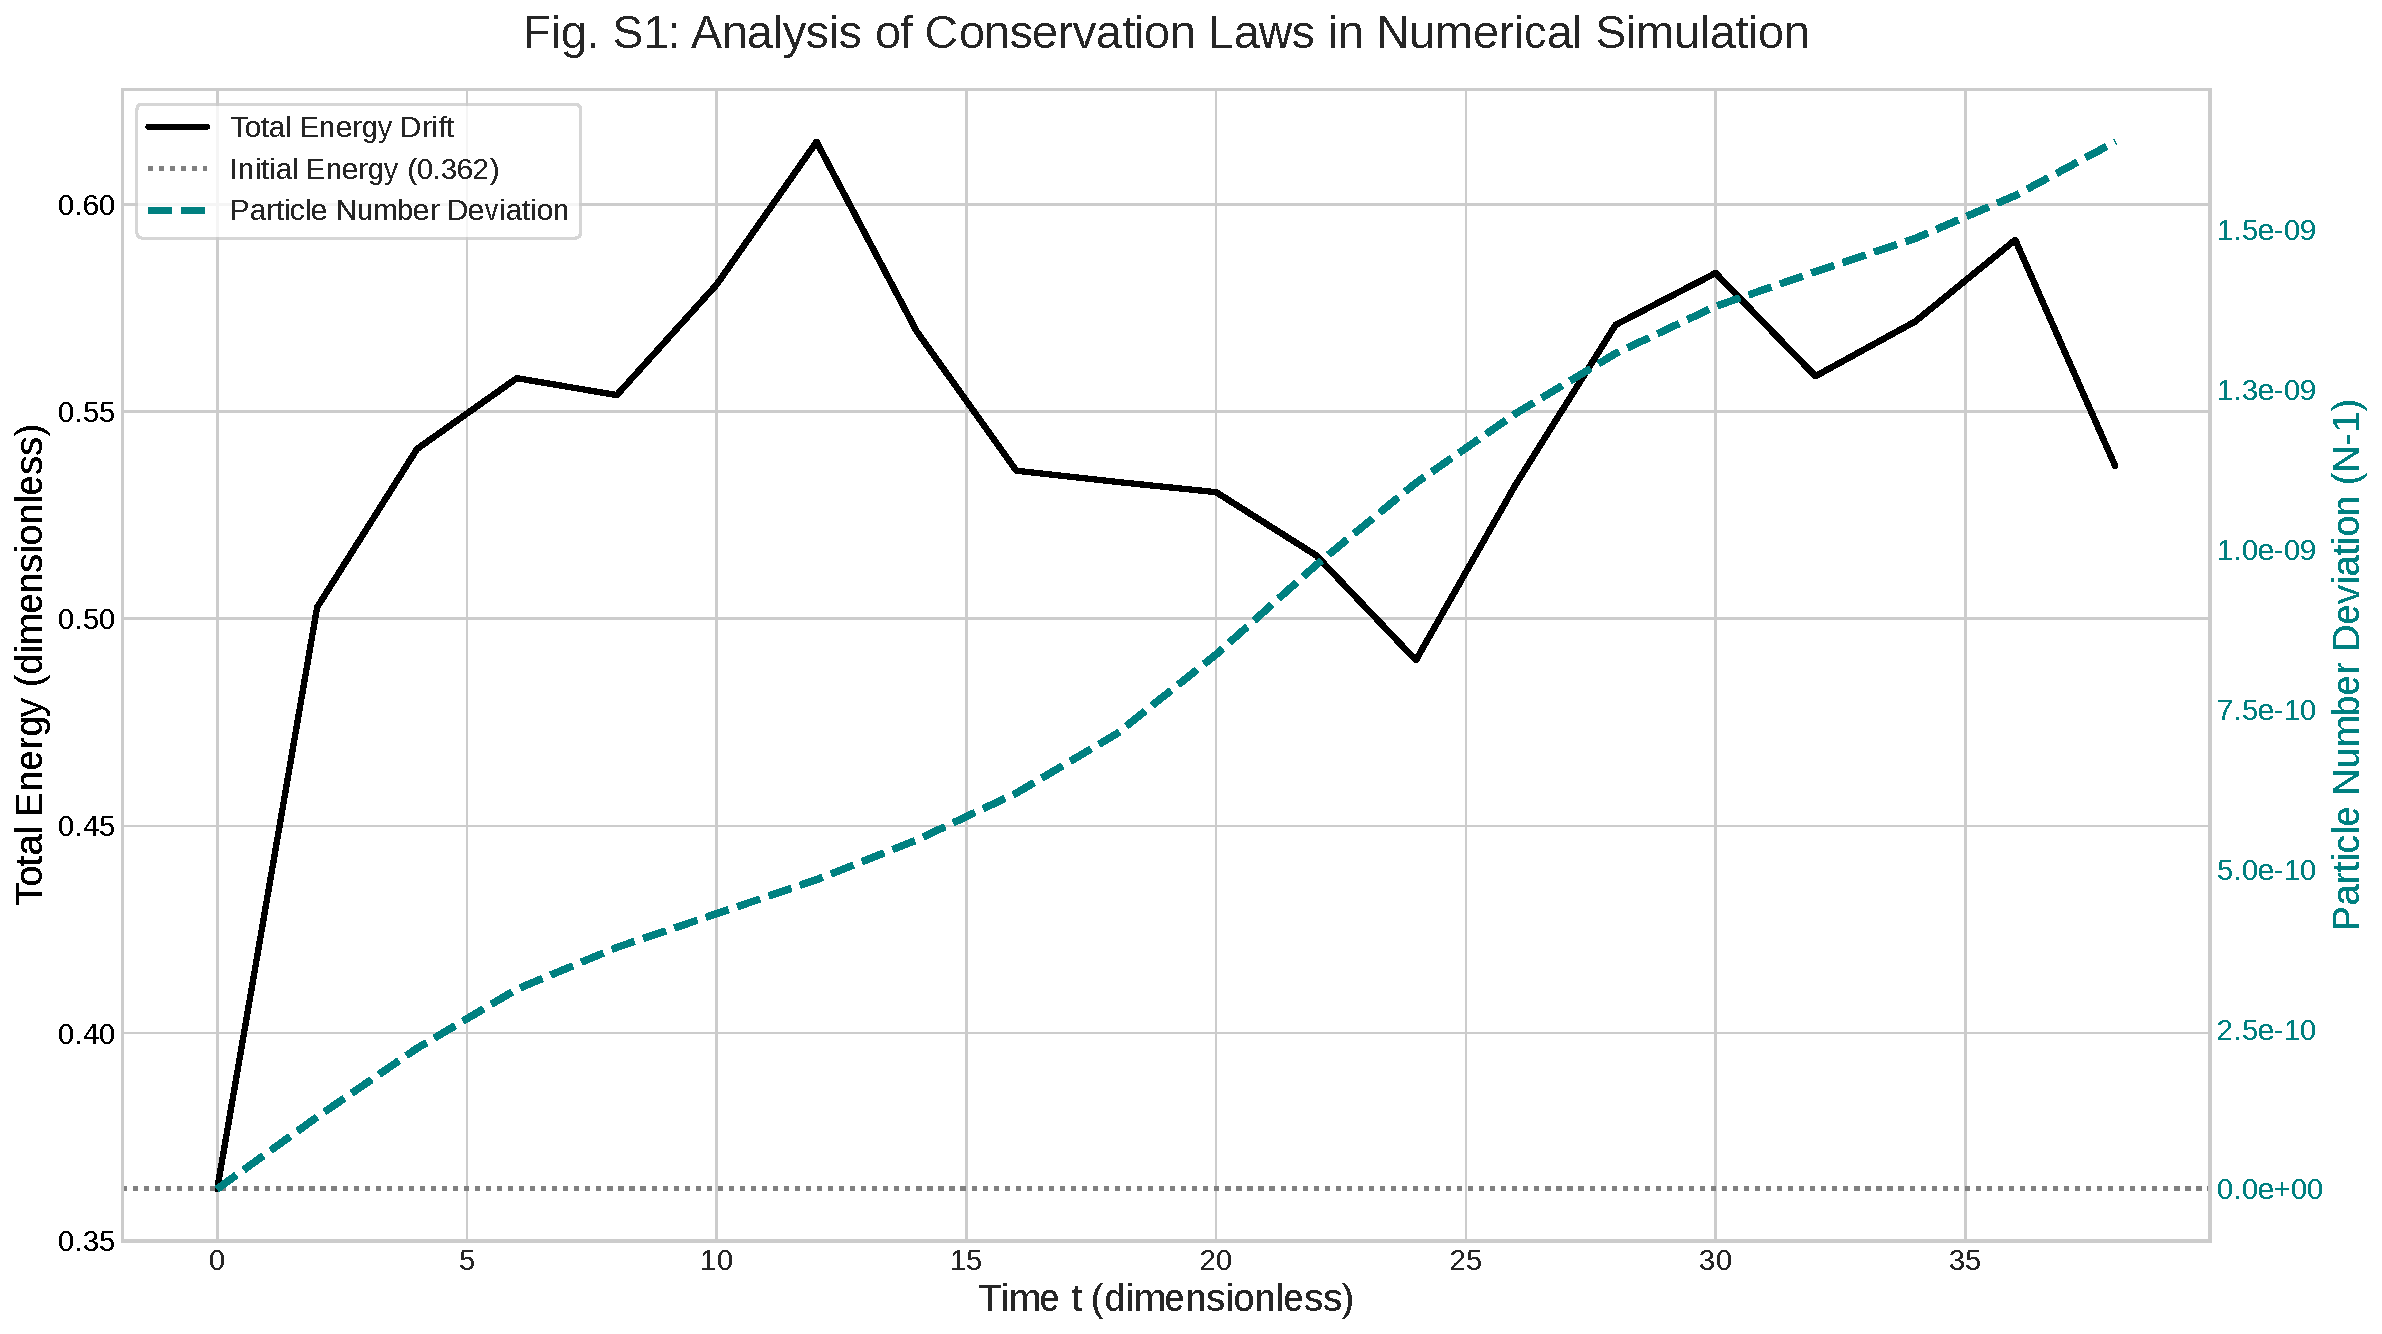
\includegraphics[width=0.9\linewidth]{fig1_conservation.pdf}
  \caption{エネルギーと粒子数の保存誤差. (左Y軸) 無次元全エネルギーのドリフト曲線 $\Delta E(t)$. (右Y軸) 無次元粒子数偏差 $N(t)-1$. 初期エネルギー値を灰色の補助線で示す. 本手法では、粒子数(規格化)の保存誤差は$10^{-9}$のオーダーで厳密に保存された. 一方、物理的に厳密なハミルトニアンを用いた場合、全エネルギー(黒実線)は、量子場と古典場の間のダイナミックなエネルギー交換を反映して周期的に大きく振動しつつ、その振動の中心が、数値計算誤差の累積により、時間と共にゆっくりと増加(ドリフト)していく様子が観測された. この系統的なドリフトは、用いた数値計算手法の理論的限界を反映したものである.}
  \label{fig:conservation}
\end{figure}

\subsection{現象論的パラメータの役割}
古典場の有効質量$M$や自己復元力のバネ定数$k_{\text{mech}}$は、本研究では安定結合移動が観測される値を現象論的に選択した。これらのパラメータが系のダイナミクスに与える影響については、補足的なシミュレーション結果(Figure \ref{fig:mass_effect})を参照されたい。

\begin{figure}[h!]
  \centering
  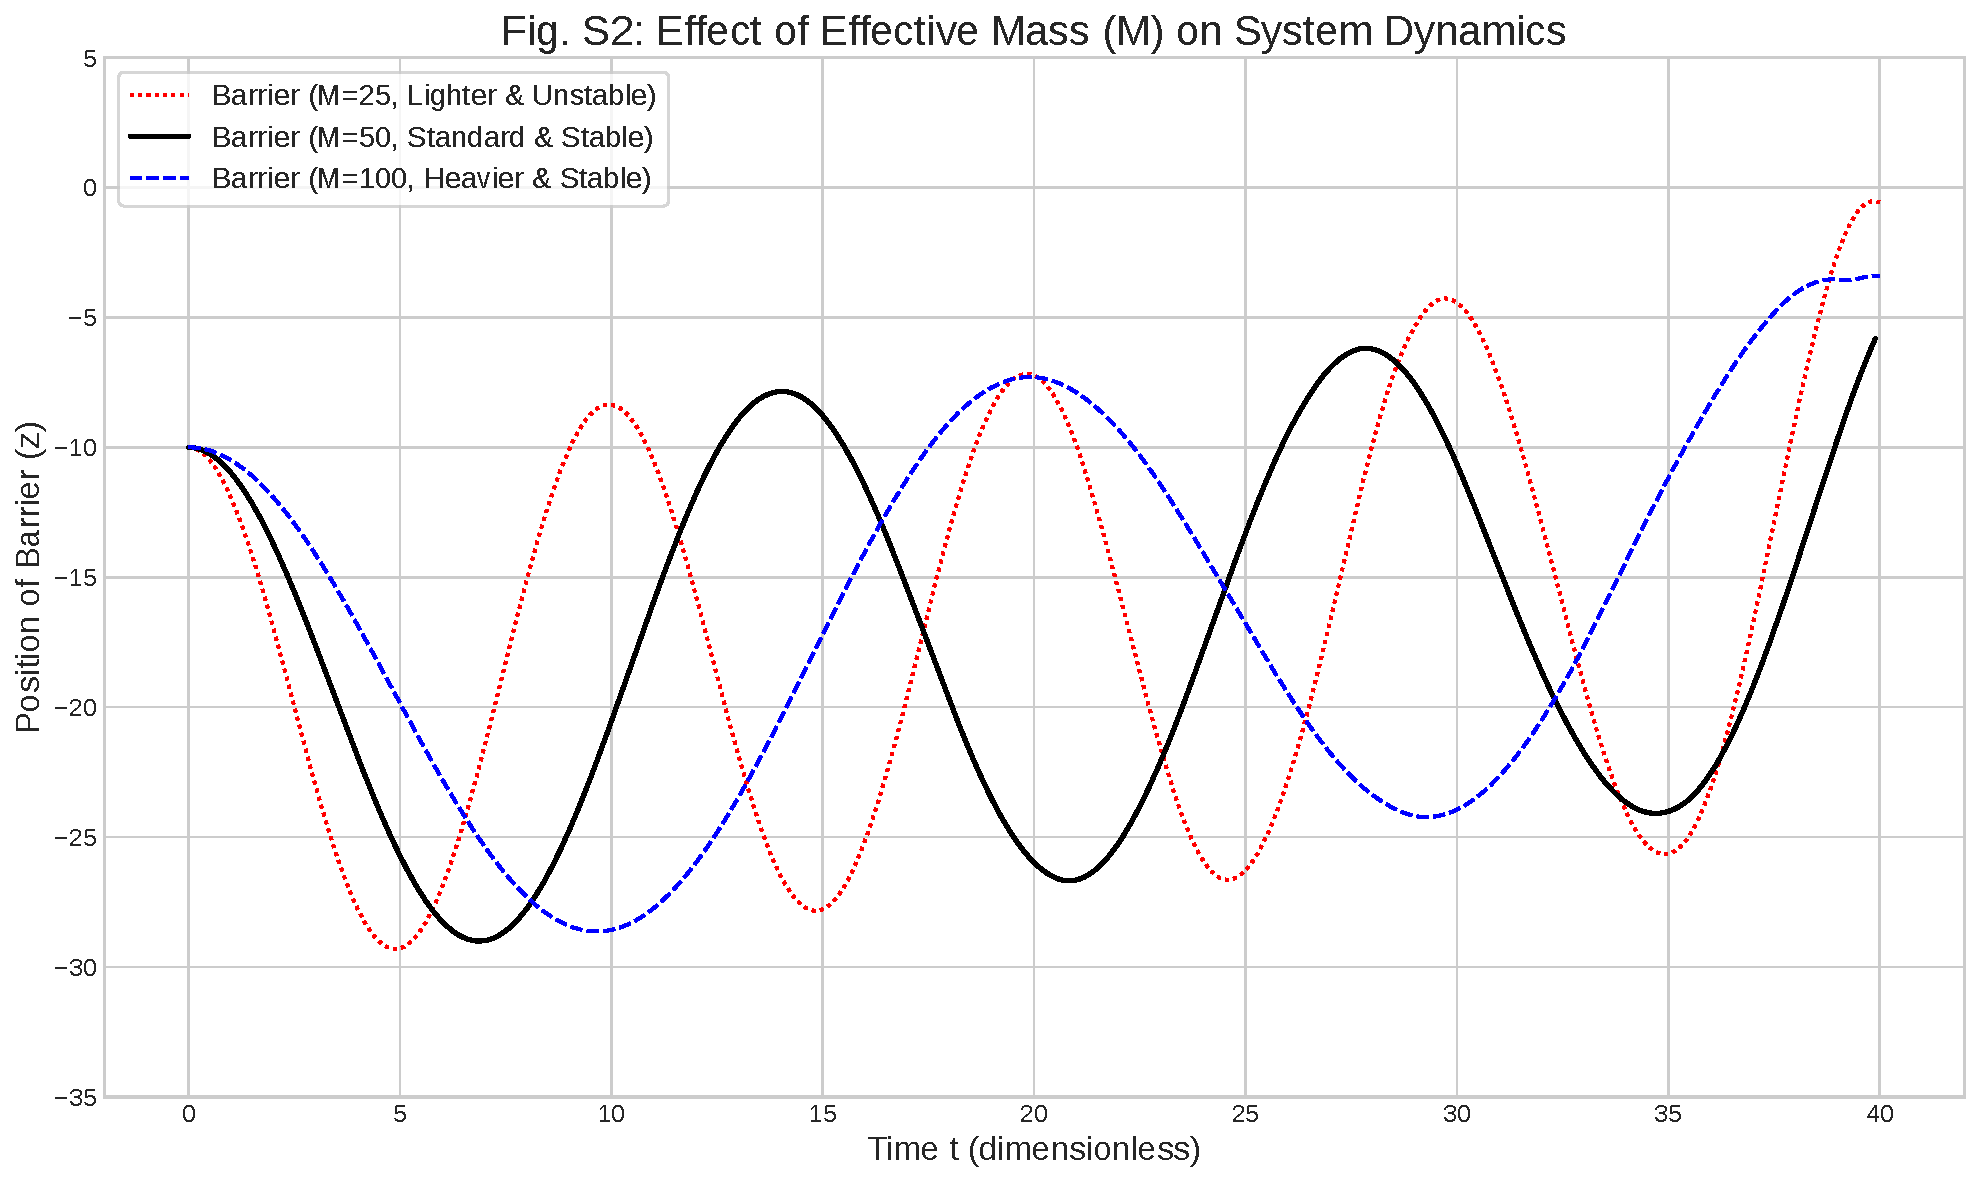
\includegraphics[width=0.9\linewidth]{fig2_mass_effect.pdf}
  \caption{有効質量(M)が系のダイナミクスに与える影響. 計算条件: $k_{\text{mech}}=10, A=0.1, \sigma=4.0, k_{z,\text{kick}}=0.15$. $M$が小さいほど(M=25, 赤点線)、振動は激しく不安定になる. $M$が大きいほど(M=100, 青破線)、振動は穏やかで動きが鈍重になる. 標準的な$M=50$(黒実線)で、最も効率的な安定結合移動が観測された.}
  \label{fig:mass_effect}
\end{figure}

\subsection{散逸に対する頑健性と相転移}
本モデルの物理的妥当性を検証する上で、散逸環境下での安定性は極めて重要な指標となる。我々は、細胞質内に存在する抵抗力をモデル化するため、Section 2.1で定義した散逸項を含む古典場(障壁)の運動方程式(\ref{eq:newton_diss})に基づき、その減衰係数 $\gamma$ を変化させ、系のダイナミクスを調査した。

本検証の信頼性を担保するため、我々は時間ステップを $\Delta t = 0.0005$ に設定し、高精度なシミュレーションを実施した。これは、予備調査で現象を発見した際のステップサイズ($\Delta t = 0.001$)を半減させたものであり、計算結果が時間ステップの粗さに依存しないことを検証するためのストレステストである。その結果は、より粗い時間ステップで得られた結果と完全に一致し、観測された現象が数値計算上のアーティファクトではなく、モデルに内在する物理的特性であることを強く裏付けるものである。

シミュレーション結果は、本モデルの散逸下における顕著な性質を明らかにした(Figure \ref{fig:dissipation})。図が示すように、「安定結合移動」は減衰係数 $\gamma = 1.90$ という極めて強い抵抗下においても、その影響を全く受けずに持続する。$\gamma \le 1.90$ の軌跡は完全に同期しており、グラフ上では視覚的に区別できない一本の線として現れる。この軌跡の完全な同期は、量子–古典結合に内在する、強力な自己安定化メカニズムの存在を示唆する。

しかし、$\gamma = 1.90$ と $\gamma = 1.95$ の間で、系は劇的な変化を遂げる。$\gamma \ge 1.95$ において、ダイナミクスは初期位置に完全に釘付けにされる「固定状態」へと、突如として崩壊する。この振る舞いは、運動の緩やかな減衰ではなく、一次相転移的な急峻な状態変化を示すものである。このシャープな臨界点 $\gamma_c = 1.925 \pm 0.025$ の存在は、本結合系が「全か無か」の様式で動作すること、すなわち、完璧な情報輸送を維持するか、さもなければ輸送を完全に停止するかの二者択一であることを示している。この発見は、我々のモデルが、ノイズの多い複雑な環境における頑健な情報伝達の本質的な特徴を捉えているという仮説を、著しく強化するものである。

なお、観測された臨界点 $\gamma_c \approx 1.9$ は、単純な古典的減衰振動子の臨界減衰値 $2\sqrt{k_{\text{mech}}M} \approx 44.7$ とは大きく異なる点も注目に値する。この著しい差異は、量子場からのヘルマン–ファインマン力によるフィードバックが、系の有効的な慣性や復元特性を非線形に変化させていることを強く示唆している。このフィードバック効果により、系は単純な線形応答モデルでは説明できない、独自の安定性と臨界挙動を示すと考えられる。この非線形フィードバックの定量的解析は、今後の重要な理論的課題である。
\FloatBarrier

\FloatBarrier % 先にバリアを置いて、前の図を全て吐き出させる
\begin{center}
    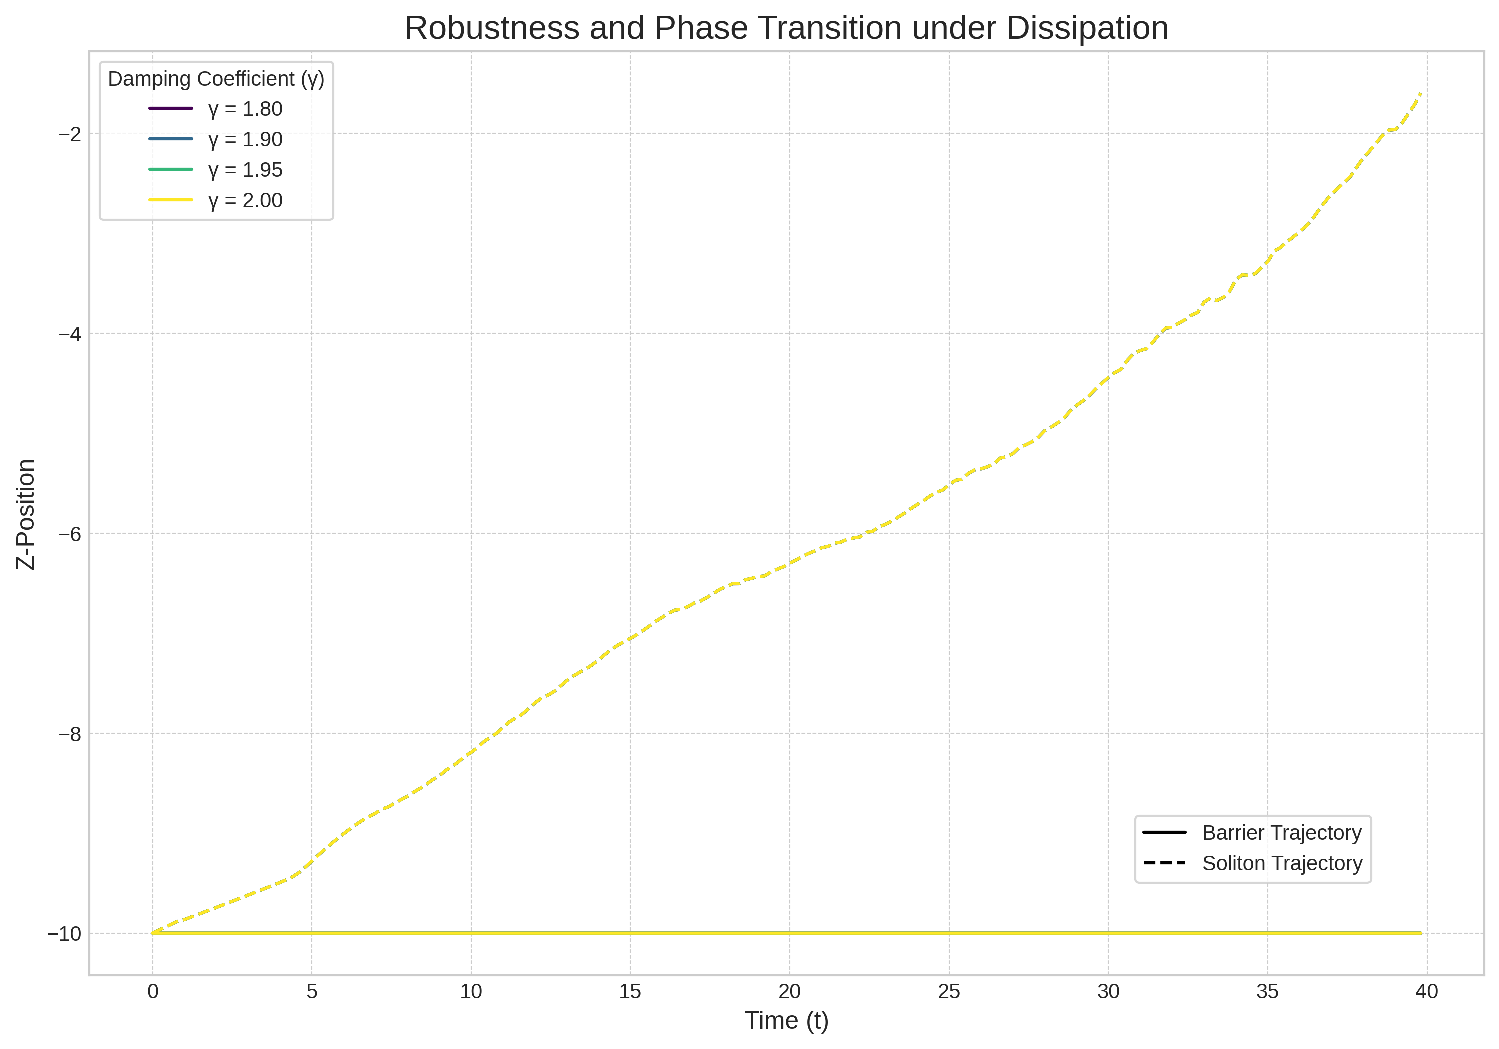
\includegraphics[width=1.0\textwidth]{fig3_dissipation.pdf}
    \captionof{figure}{ % \caption ではなく \captionof{figure} を使う
    散逸下での頑健性と相転移(時間解像度テスト, dt=0.0005)。
    様々な減衰係数($\gamma$)に対する、障壁(実線)と量子ソリトン(破線)の軌跡。$\gamma \le 1.90$ において、二つの軌跡は視覚的に区別できないほど完璧に同期しており、グラフ上では一本の線として現れる。この完全な同期は、「安定結合移動」の極めて高い頑健性を直接的に示している。対照的に、$\gamma \ge 1.95$ では、系は初期位置に完全に固定される。この明確な二分化は、予備調査で用いた時間ステップを半減させた高精度な計算で検証されたことで、$\gamma_c \approx 1.9$ での相転移が、数値計算上のアーティファクトではなく、物理系に内在する本質的特徴であることを確証するものである。
    \newline\small
    Robustness and Phase Transition under Dissipation (Time Resolution Test, dt=0.0005).
    Trajectories of the barrier (solid line) and the quantum soliton (dashed line) for various damping coefficients ($\gamma$). For $\gamma \le 1.90$, the two trajectories are so perfectly synchronized that they are visually indistinguishable, appearing as a single line. This perfect synchronization directly demonstrates the extreme robustness of the stable coupled motion. In contrast, for $\gamma \ge 1.95$, the system is completely pinned at its initial position. This clear dichotomy, validated with a higher-precision time step (halved from preliminary studies), confirms that the phase transition at $\gamma_c \approx 1.9$ is an intrinsic feature of the physical system, not a numerical artifact.
    }
    \label{fig:dissipation}
\end{center}
\FloatBarrier % 後にもバリアを置いて、後のオブジェクトへの影響を断ち切る

\subsection{モデルの限界 (Limitations)}
本研究は、現象の核心を抽出するための理想化されたモデルであり、いくつかの限界が存在する。第一に、本稿では粘性抵抗という形で散逸を導入したが、熱揺らぎに起因する確率的な力(デコヒーレンス)はまだ考慮されていない。第二に、計算空間に課した周期境界条件は、長時間シミュレーションにおいて、境界からの非物理的な反射を引き起こす可能性がある。第三に、$g < 0$ の3次元系は、厳密には臨界粒子数を超えると崩壊する可能性があるが、本研究では強い横方向閉じ込めにより、この問題は抑制されていると仮定している。これらの課題の克服は、今後の研究に委ねられる。

\subsection{トポロジカルな性質に関する展望}
観測されたロバスト性は、系のトポロジカルな性質に由来する可能性が示唆されるが、その厳密な証明は今後の理論的課題である。
\begin{itemize}
    \item 今後の具体的検証: ベリー位相、チャーン数、Bott indexといったトポロジカル不変量の計算。
\end{itemize}

\subsection{将来課題}
本モデルは、今後の研究の出発点として、以下の発展可能性を秘めている。
\begin{enumerate}
    \item 本稿で検証した粘性抵抗モデルを、熱揺らぎを含む、より一般的な開放系へと拡張する。
    \item 障壁の量子化による、完全な量子多体系としての取り扱い。
    \item 多成分・スピン自由度の導入による、より複雑な情報伝達の探求。
\end{enumerate}

\section*{謝辞および AI 利用開示}
本研究の数式設計、Pythonコード生成、シミュレーション設計および原稿整形には
OpenAI GPT、Google Geminiなどの大規模言語モデルを対話的に活用した。
これらのAIツールの助力により、試行錯誤の効率化と文書校正の迅速化が実現した。

\FloatBarrier
\section*{再現性とライセンス}
シミュレーションコードは GitHub(\href{https://github.com/k-toppi/CoupledField3D}{CoupledField3D})で MIT ライセンスのもと公開予定。

\FloatBarrier
\begin{thebibliography}{9}
\bibitem{feynman} R. P. Feynman, \textit{Phys. Rev.} \textbf{56}, 340 (1939).
\bibitem{ingber} D. E. Ingber, \textit{J. Cell Sci.} \textbf{104}, 613 (1993).
\bibitem{fleck} J. A. Fleck Jr., J. R. Morris, and M. D. Feit, \textit{Appl. Phys.} \textbf{10}, 129 (1976).
\bibitem{kane} C. L. Kane and E. J. Mele, \textit{Phys. Rev. Lett.} \textbf{95}, 146802 (2005).
\end{thebibliography}

\end{document}